\subsection{Determinant of Hessian}
Determinant of Hessian eller \textit{DoH}: $\textbf{det}\mathcal{H}L$ , udgør feature detektoren i
SURF. DoH er baseret på Hessian matricen, som udregnes for hvert punkt $p=(x,y)$ i et billede:
\begin{equation}
\mathcal{H}(p, \sigma) = 
 \begin{bmatrix}
 	L_{xx}(p, \sigma) & L_{xy}(p, \sigma) \\
 	L_{xy}(p, \sigma) & L_{yy}(p, \sigma) 
 \end{bmatrix}
 \label{hessianmatrix}
\end{equation}
hvor $\sigma$ svarer til skalaen og $L_{xy} $, $L_{yy}$ og $L_{xx}$\eqref{lxx}, er den Gaussiske funktionen, partielt differentieret ifht. $xy$, $yy$ og $xx$.
\begin{equation}
L_{xx}(x, \sigma) = (\frac{\partial^2 }{\partial x^2 } G(x,y,\sigma)) * I
\label{lxx}
\end{equation}
Bay et.al anvender approkismerede, vægtede box filtrer $D_{xx}$, $D_{yy}$ og $D_{xy}$, der ved brug af integralbilleder nedsætter antallet af beregninger drastisk. Disse filtrer består udelukkende af værdier af -2,-1,0 eller 1. I implementeringen er disse boxfiltrer ikke anvendt, og er derved udregnet som i \eqref{lxx}, figur \ref{fig:lxxlyylxy} viser en illustration af de anvendte filtre.
\begin{figure}[H]
    \centering
    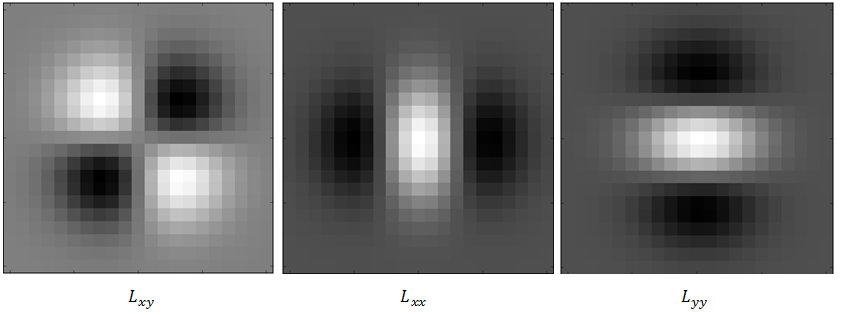
\includegraphics[width=0.75\textwidth]{fig/31.png}
     \vspace{-0.5em}
    \begin{center}    
       \caption{\textcolor{gray}{\footnotesize \textit{ }}}
    \label{fig:lxxlyylxy}
     \end{center}
     \vspace{-2.5em}
  \end{figure} \noindent
I metoden oprettes skalarummet ved iterativt at forøge størrelsen af filtrene, med $\sigma=1.2$, fremfor at forøge størrelsen af $\sigma$. For hver oktav, eksisterer, i denne implementering, fire billeder, foldet med fire forskellige filterstørrelser. For hver oktav, bruges nr. to filterstørrelse, fra forrige oktav til starten af den næste oktav, og størrelsen imellem filtre, fordobles fra forrige oktav, som vist i tabel \ref{fig:secderivfiltersize}. Her skal det bemærkes, at de andenafledte filtre, skal have dobbelt størrelse, af de førsteafledte, som er vist i tabel \ref{fig:firstderivfiltersize}
\begin{figure}[H]
    \centering
    \begin{center}    
    \begin{tabular}{ | l | l | l | l | l |}
    \hline
    oktav & filter str 1 & filter str 2 & filter str 3 & filter str 4 \\ \hline
    1 & 9 & 15 & 21 & 27 \\ \hline
  	2 & 15 & 27 & 39 & 51 \\ \hline
  	3 & 27 & 51 & 75 & 99 \\ \hline
  	4 & 51 & 99 & 147 & 195 \\ \hline
    \end{tabular}       
    \caption{\textcolor{gray}{\footnotesize \textit{Fire forskellige oktaver, og filterstørrelse, for et andenafledt filter}}}
    \label{fig:secderivfiltersize}
     \end{center}
     \vspace{-2.5em}
  \end{figure} \noindent
For hvert punkt i billederne opstilles Hessian matricen, hvorefter determinten udregnes for alle punkter i billederne. Bay et.al. udregner determinanten ved:
\begin{equation}
\textbf{det}\mathcal{H}_{approksimeret} = D_{xx}D_{yy}-wD_{xy}^2
\label{deerminantofhessian}
\end{equation}
, hvor $w$ er en vægt, tilføjet, for at balancere de approksimerede filtre og boks filtrene. Da denne implementering ikke anvender boks filtrer udregnes determinanten som:
\begin{equation}
\textbf{det}\mathcal{H} = L_{xx}L_{yy}-L_{xy}^2
\label{deerminantofhessian}
\end{equation}
Determinant of Hessian reagere på mørke og lyse blobs, ved positive svar. Derfor udvælges et lokalt maxima af et $3\times3\times3$ område af determinantbillederne, som vist på figur \ref{fig:difference}. Dette udføres for alle oktaver. Herefter udvælges korrekt subpixel placering, hvilket er en metode introduceret af David Lowe, også beskrevet i SIFT. Igen udføres dette skridt ved at fjerne punkter ikke lokaliseret tæt nok på ekstremaer og svage ekstremaer.
\subsection*{Algoritme}
\begin{enumerate}
\item {Hessian matricen opstilles for alle punkter i skalabillederne som:
$$
\mathcal{H} = 
 \begin{bmatrix}
 	L_{xx} & L_{xy} \\
 	L_{xy} & L_{yy} 
 \end{bmatrix} $$
}
\item Determinantbilleder opstilles, ved at udregne determinanten af Hessian matricen for alle punkter i alle billeder ved:
$$
\textbf{det}\mathcal{H} = L_{xx}L_{yy}-L_{xy}^2
$$
\item Lokale maxima udvælges, af hvert $3\times3\times3$ område af billeder på samme oktav.
\item Accurate keypoint localisation, bruges til at fjerne dårligt lokaliserede punkter.
\end{enumerate}